\documentclass[a4paper]{article}

\usepackage[hidelinks]{hyperref}
\usepackage{siunitx}
\usepackage[a4paper, margin=1in]{geometry}
\usepackage{graphicx}
\usepackage{tikz}
\usepackage{circuitikz}
\usepackage{pgfplots}
\pgfplotsset{width=10cm, compat=newest}
\usetikzlibrary{decorations.pathmorphing}
\usetikzlibrary{quotes,arrows.meta}
\usetikzlibrary{patterns}
\usepackage{amsmath}
\usepackage{setspace}
\usepackage{subcaption}
\usepackage[notquote]{hanging}
\usepackage{setspace}
\usepackage{pdflscape}

\tikzset{
   ragged border/.style={ decoration={random steps, segment length=1mm, amplitude=0.5mm},
           decorate,
   }
}

\newsavebox{\battery}
\sbox{\battery}{
  \begin{circuitikz}[sharp corners, european]
    \draw (0,0) to [battery,*-*] (4,0);
    \node at (2, 0.75) {V};
  \end{circuitikz}
}

\tikzset{
  annotated cuboid/.pic={
    \tikzset{%
      every edge quotes/.append style={midway, auto},
      /cuboid/.cd,
      #1
    }
    \draw [every edge/.append style={pic actions, densely dashed, opacity=.5}, pic actions]
    (0,0,0) coordinate (o) -- ++(-\cubescale*\cubex,0,0) coordinate (a) -- ++(0,-\cubescale*\cubey,0) coordinate (b) edge coordinate [pos=1] (g) ++(0,0,-\cubescale*\cubez)  -- ++(\cubescale*\cubex,0,0) coordinate (c) -- cycle
    (o) -- ++(0,0,-\cubescale*\cubez) coordinate (d) -- ++(0,-\cubescale*\cubey,0) coordinate (e) edge (g) -- (c) -- cycle
    (o) -- (a) -- ++(0,0,-\cubescale*\cubez) coordinate (f) edge (g) -- (d) -- cycle;
    \path [every edge/.append style={pic actions, |-|}]
    (b) +(0,-5pt) coordinate (b1) edge ["\cubex \cubeunits"'] (b1 -| c)
    (b) +(-5pt,0) coordinate (b2) edge ["\cubey \cubeunits"] (b2 |- a)
    (c) +(3.5pt,-3.5pt) coordinate (c2) edge ["\cubez \cubeunits"'] ([xshift=3.5pt,yshift=-3.5pt]e)
    ;
  },
  /cuboid/.search also={/tikz},
  /cuboid/.cd,
  width/.store in=\cubex,
  height/.store in=\cubey,
  depth/.store in=\cubez,
  units/.store in=\cubeunits,
  scale/.store in=\cubescale,
  width=10,
  height=10,
  depth=10,
  units=cm,
  scale=.1,
}

\tikzset{
  cuboid/.pic={
    \tikzset{%
      every edge quotes/.append style={midway, auto},
      /cuboid/.cd,
      #1
    }
    \draw [every edge/.append style={pic actions, densely dashed, opacity=.5}, pic actions]
    (0,0,0) coordinate (o) -- ++(-\cubescale*\cubex,0,0) coordinate (a) -- ++(0,-\cubescale*\cubey,0) coordinate (b) edge coordinate [pos=1] (g) ++(0,0,-\cubescale*\cubez)  -- ++(\cubescale*\cubex,0,0) coordinate (c) -- cycle
    (o) -- ++(0,0,-\cubescale*\cubez) coordinate (d) -- ++(0,-\cubescale*\cubey,0) coordinate (e) edge (g) -- (c) -- cycle
    (o) -- (a) -- ++(0,0,-\cubescale*\cubez) coordinate (f) edge (g) -- (d) -- cycle;
  },
  /cuboid/.search also={/tikz},
  /cuboid/.cd,
  width/.store in=\cubex,
  height/.store in=\cubey,
  depth/.store in=\cubez,
  units/.store in=\cubeunits,
  scale/.store in=\cubescale,
  width=10,
  height=10,
  depth=10,
  units=cm,
  scale=.1,
}

\begin{document}

\title{The relationship between the voltage during a process of anodizing and
the thickness of the anodized layer}
\author{Marko Vejnovi\'{c}}

\maketitle

\doublespacing

\section*{Rationale}
\paragraph*{}
Regarding chemistry overall, I am most interested in industrial chemistry. Due
to my affinity for physics and engineering, I am naturally drawn to everything
regarding engineering, including industrial chemistry. As I was thinking about
a topic for my Chemistry Internal Assessment, I oversaw my roommate's
\textit{FiiO E10K} (``E10K''). The \textit{FiiO E10K} is a device covered in
anodized aluminum. I thought about how I never actually learned how anodized
aluminum is made, and therefore I decided to conduct my research in the field
of anodizing.

\section{Introduction}
\paragraph*{}
In contact with atmospheric contents, aluminum surface becomes quickly coated
with a layer of aluminum oxide with a thickness of up to $1-2\si{\micro
m}$. Because of the low thickness of the aluminum oxide, high porosity and low
mechanical strength, this oxide layer does not protect the aluminum in any
significant amount (Ardelean, Marius and Lascău, S and Ardelean, Erika and
Josan, Ana).

\paragraph*{}
However, a sufficiently thick superficial oxide layer does prove to be both
protective and aesthetically pleasing. Through the process of anodic oxidation,
a thicker, around $20$ to $50\si{\micro m}$, oxide film can be achieved. These
artificial films are more mechanically stable, heat-resistant, porous, stable
to water vapor and other corrosive agents, compared to their natural
counterparts (Ardelean, Marius and Lascău, S and Ardelean, Erika and Josan,
Ana). This process of artificial induction of the oxide layer is referred to as
the process of \textit{hard anodizing} (Sheasby, P. G.; Pinner, R.).

\begin{figure}[ht]
  \centering
  \includegraphics[width=0.4\textwidth]{img/clralu}
  \caption{An example of an anodized aluminum sheet (KI)}
  \label{fig:clr-alu-anodized}
\end{figure}

\paragraph*{}
The process of anodizing has two main purposes - increasing the resistance to
corrosion as well as decoration. The resistance to corrosion stems from the
fact that the oxide layer cannot corrode. Anodized aluminum can be dyed making
the oxide film decorative as well as protective.

\begin{figure}[ht]
  \centering
  \includegraphics[width=0.4\textwidth]{img/coloralu}
  \caption{An example of colorful anodized aluminum parts (Fischer)}
  \label{fig:color-alu-anodized}
\end{figure}

\subsection{The anodizing process}

\paragraph*{}
The process of forming aluminum oxide film is a redox reaction which occurs in
an electrochemical cell as shown in figure \ref{fig:ec-cell}.

\begin{figure}[ht]
  \centering
  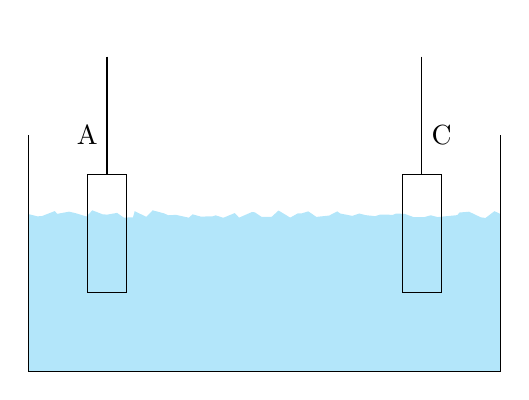
\begin{tikzpicture}
    \fill[cyan!30]
        decorate[ragged border]{
          (-3,2) -- (3,2)
        } -- (3,0) -- (-3,0) -- cycle;

    \draw (-3,3) -- (-3,0) -- (-3,0) -- (3,0) -- (3,3);

    \node at (0, 4.25) {\usebox{\battery}};

    \draw (-2, 4) -- (-2, 2.5);
    \draw (-2.25, 2.5) -- (-1.75, 2.5) -- (-1.75, 1) -- (-2.25, 1) -- cycle;

    \draw (2, 4) -- (2, 2.5);
    \draw (2.25, 2.5) -- (1.75, 2.5) -- (1.75, 1) -- (2.25, 1) -- cycle;

    \node at (-2.25, 3) {A};
    \node at (2.25, 3) {C};

  \end{tikzpicture}
  \caption{The anodizing electrochemical cell}
  \label{fig:ec-cell}
\end{figure}

\paragraph*{}
Aluminum is used as the anode $A$ as it will oxidize. The cathode $C$ is a
chemically inert electrode such as carbon or lead. The electrolyte can be
chosen at will, however for a thick coating of aluminum oxide a strong acid
proves to be more effective. When voltage $V$ is applied an electrolysis
reaction occurs. The following two reactions happen at the cathode $C$ and the
anode $A$:
\begin{align*}
  A: 2Al + 3H_2O &\rightarrow Al_2O_3 + 6H^+ + 6e^- \\
  C: 6H^+ + 6e^- &\rightarrow 3H_2
\end{align*}

\paragraph*{}
The resulting anodizing reaction is:
$$2Al + 3H_2O \rightarrow Al_2O_3 + 3H_2$$

\subsection{The growth mechanism}

\paragraph*{}
The oxide film comes in two forms - a barrier type film and a porous type film
(Ono), as shown in figure \ref{fig:ono-films}. The barrier type film is the one
naturally most occurring while the porous type film is the one which is usually
formed by anodizing. The barrier type film is a homogeneous sheet of $Al_2O_3$,
while the porous type film has small holes in which molecules fit. These small
holes can be filled with dye molecules making the object colorful\footnote{It
is interesting to note that anodized aluminum parts never come in the color
white because of the fact that white dye (leuco dye) molecules are larger than
the pores and therefore cannot fit inside the pores.}.

\begin{figure}[ht]
  \centering
  \includegraphics[width=0.6\textwidth]{img/ono-films}
  \caption{The two types of $Al_2O_3$ oxide film (Ono)}
  \label{fig:ono-films}
\end{figure}

\paragraph*{}
The formation of the oxide layer is as follows. At a constant power generated
by a voltage generator, the relationships between the anodizing time and the
voltage and current density are given in figure \ref{fig:ono-relationship}. The
separate stages are represented in the figure. From stage $I$ to $II$ the
barrier type film is formed. As the anodizing process continues, the voltage
will increase. Between stages $II$ and $III$, as the film grows, grooves will
become etched in it. Between stage $III$ and $IV$, pores will start forming.

\begin{figure}[ht]
  \centering
  \includegraphics[width=0.6\textwidth]{img/ono-relationship}
  \caption{The formation of the porous oxide film (Ono)}
  \label{fig:ono-relationship}
\end{figure}

\subsection{Impact of voltage}

\paragraph*{}
The voltage applied during the anodizing process heavily impacts the thickness
of anodized layer. Since the thickness of the anodized layer heavily impacts
the \textit{Vickers hardness}\footnote{A measure of a material's resistance to
plastic deformation - irreversible changes to its shape} of the overall
aluminum, it is important to be able to predict the thickness of the film with
respect to the voltage applied for a constant time.

\paragraph*{}
Therefore, the research question of this paper is: \textit{What is the
  relationship between the voltage applied during the process of aluminum
anodizing and the thickness of the anodized film?}

\paragraph*{}
It was hypothesized that the relationship between the voltage and the thickness
of the anodized film to be logarithmically dependent - as the voltage
increases, more of the film will form. However, as more of the film forms the
electrical resistance will increase, decreasing the rate of anodizing.

\subsection{Significance}

\paragraph*{}
Research in this field could prove useful in consumer products. Anodized
aluminum products are very common and products with a maximal hardness would be
most resistant to scratching and other day-to-day material deformations.
Moreover, since the thickness of the oxidized film impacts how resistant
aluminum is to corrosion, research in the field could prove useful to both the
automotive and the aeronautical industries as it would enable better prediction
of the behavior of the industries' products.

\section{Method}

\subsection{Anodizing} \label{sec:anodizing}

\subsubsection{Cleaning}

\paragraph*{}
Before the actual anodizing reaction, it is necessary to clean the aluminum
bars that are to be anodized. First they are cleaned using a detergent to
remove any oils that may be present. After that, they are settled in a solution
of $NaOH$ for about $3$ minutes. The reaction that occurs is:
$$Al_2O_3 + 2NaOH + 3H_2O \rightarrow 2Na[Al(OH)_4]$$
This reaction cleans off the already existing oxide film.

\subsubsection{Anodizing reaction}

\paragraph*{}
The anodizing process can be done as follows. In a  250$\si{ml}$ beaker, dilute
sulfuric acid is carefully poured. The positive side of a lab bench power
supply is connected to an aluminum rod. The negative side of the power supply
is connected to a graphite cathode. These are both submerged in the sulfuric
acid. The voltage is applied and the electrolysis process starts. The process
is conducted for a fixed time after which the aluminum rod is pulled out of the
solution.

\subsubsection{Tempering}

\paragraph*{}
After the process of anodizing, the aluminum rod is put in boiling water for
around $15$ minutes and then cooled off to room temperature, which allows the
newly formed film to temper itself.

\subsection{Thickness of the film}

\paragraph*{}
Measuring the thickness of the oxide film is nearly impossible with
conventional methods of using a caliper and micrometer. Calipers are not
precise enough to measure the thickness of the film layer, and a micrometer is
too precise to use multiple times accurately. As such, it is necessary to
develop a different method which will enable the measurement of the layer.

\paragraph*{}
In this paper, a different method if proposed. Instead of directly measuring
the thickness of the anodized layer, it is proposed to measure the change in
mass before the anodizing process and after it. With a sufficiently precise
scale, it is, in theory, possible to accurately estimate the thickness of the
film.

\paragraph*{}
The method for estimating the thickness of the anodized layer is as follows.
First, the mass of the un-anodized aluminum $m_0$ is measured. This is to be
done immediately before the process of the anodizing reaction. After the
reaction and the tempering, the mass of the anodized aluminum $m_1$ is
measured. Since the process under which aluminum undergoes is
$$2Al \rightarrow Al_2O_3$$
and since it is reasonable to assume that all of the $Al_2O_3$ will reside on
the walls of the $Al$, it can be inferred that:
\begin{align*}
  m_1 &= m_0 + m(O) \\
  m_1 &= m(Al_2O_3) + m_0 - m(Al)
\end{align*}
The mass of the aluminum can be calculated as follows. Since the mass of oxygen
is known ($m(O) = m_1 - m_0$), the number of moles of oxygen is also
calculable:
$$n(O) = \frac{m(O)}{M(O)}$$
Since there are $3$ oxygen atoms in every molecule of $Al_2O_3$, it follows
that:
\begin{align*}
  n(Al_2O_3) &= \frac{1}{3} n(O) \\
  &= \frac{1}{3} \cdot \frac{m(O)}{M(O)}
\end{align*}
and then:
\begin{align*}
  m(Al_2O_3) &= n(Al_2O_3) \cdot M(Al_2O_3) \\
  &= \frac{1}{3} \cdot \frac{m(O)}{M(O)} \cdot M(Al_2O_3)
\end{align*}
The volume of $Al_2O_3$ is then:
\begin{align*}
  V(Al_2O_3) &= \frac{m(Al_2O_3)}{\rho(Al_2O_3)} \\
  &= \frac{1}{3} \cdot \frac{m(O)}{M(O)} \cdot M(Al_2O_3) \cdot
    \frac{1}{\rho(Al_2O_3)}
\end{align*}

\subsubsection{Thickness calculation} \label{sec:thickness-calculation}

\paragraph*{}
Finally, to calculate the thickness of the anodized layer, the following method
is employed. Let us first assume that the oxide film is uniform. Consider the
modeled $Al$ bar given in figure \ref{fig:al-bar}. The $Al$ bar is given in
black, and the oxide film is given in blue. Let us denote the dimensions of the
$Al$ bar as: $a$, $b$ and $c$. The thickness (the distance from the edge of the
aluminum to the edge of the oxide film) is $t$.

\begin{figure}[ht]
  \centering
  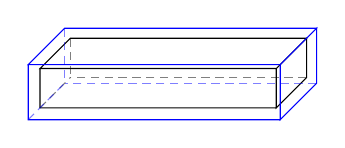
\begin{tikzpicture}
    \pic [] at (-0.05,-0.05) {cuboid={width=30, height=5, depth=10}};
    \pic [draw=blue] at (0,0) {cuboid={width=32, height=7, depth=12}};
  \end{tikzpicture}
  \caption{A model of the anodized $Al$ bar}
  \label{fig:al-bar}
\end{figure}

If the assumption is made that the oxide film grows around the aluminum bar
during anodizing, then the volume can be expressed as:
\begin{align*}
  (a + t)(b + t)(c + t) &= V_{Al_2O_3} + V_{Al} \\
  abc + t^3 + (a + b + c) \cdot t^2 + (ab + ac + bc) \cdot t &= V_{Al_2O_3} +
  V_{Al} \\
  t^3 + (a + b + c) \cdot t^2 + (ab + ac + bc) \cdot t &= V_{Al_2O_3} \\
  t^3 + (a + b + c) \cdot t^2 + (ab + ac + bc) \cdot t - V_{Al_2O_3} &= 0 \\
\end{align*}
The solutions for the cubic equation can be computationally achieved.

\subsubsection{A more accurate model} \label{sec:accurate-model}

\paragraph*{}
Note that the aforementioned model is not perfect as it does not consider the
fact that aluminum on the bar depletes becoming $Al_2O_3$. Refer to figure
\ref{fig:micro-al-bar} for a microscopic view of a model which does consider
this. The following notation is used: $t$ is the thickness of the oxide film,
$d$ is the equivalent thickness to the oxygen molecules that oxidized, $l$ is
the equivalent thickness of aluminum that oxidized and $a$ is the width of the
bar. This method is not employed due to its difficulty.

\begin{figure}[ht]
  \centering
  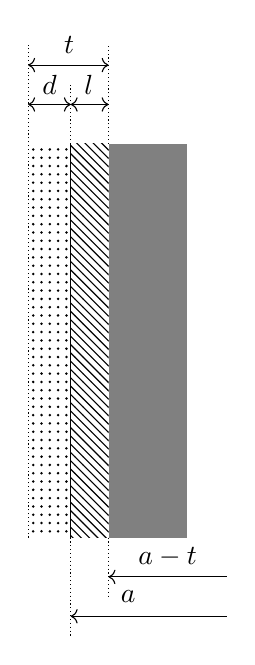
\begin{tikzpicture}
    \fill [gray] (0.5,0.25) rectangle (1.5,5.25);
    \fill [pattern=north west lines] (0.02,0.25) rectangle (0.5,5.25);
    
    \fill [pattern=dots] (-0.52, 0.25) rectangle (0.02, 5.25);

    \draw (0.02,5.25) -- (0.02,0.25);

    \draw [densely dotted] (0.5, 5.25) -- (0.5, 6.5);
    \draw [densely dotted] (0.02, 5.25) -- (0.02, 6);
    \draw [densely dotted] (-0.52, 0.25) -- (-0.52, 6.5);

    \draw [<->] (0.02,5.75) -- (0.5,5.75);
    \draw [<->] (-0.52,5.75) -- (0.02, 5.75);
    \draw [<->] (-0.52,6.25) -- (0.5, 6.25);

    \node at (0.25, 6) {$l$};
    \node at (-0.25, 6) {$d$};
    \node at (0, 6.5) {$t$};

    \draw [densely dotted] (0.02,0.25) -- (0.02, -1);
    \draw [densely dotted] (0.5,0.25) -- (0.5,-0.5);

    \draw [<-] (0.5,-0.25) -- (2,-0.25);
    \draw [<-] (0.02,-0.75) -- (2,-0.75);

    \node at (0.75,-0.5) {$a$};
    \node at (1.25,0) {$a-t$};

  \end{tikzpicture}
  \caption{A microscopic view of the anodized $Al$ bar}
  \label{fig:micro-al-bar}
\end{figure}
The method mentioned in section \ref{sec:thickness-calculation} allows only for
calculating $d$ and does not take into account that $l$ also plays a role in
$t$. In mathematical terms, section \ref{sec:thickness-calculation} assumes that
$t = d$. However, it is impossible, with the methods described previously, to
calculate the thickness of the anodized layer with the assumption that $t = d +
l$.

\subsection{Hazards and safety precautions} \label{sec:safety}

\paragraph{Sulfuric acid}
Sulfuric acid is highly corrosive and cause severe skin and eye damage. It is
also highly damaging to the environment. It must be used with appropriate eye
and skin protection, as well as have a neutralizer readily available in case of
spillage. It is to be disposed according to the institution's regulations for
disposing acid.

\paragraph{Sodium hydroxide}
A solution of $NaOH$ is severely damaging to skin and eyes. As with sulfuric
acid, proper eye and skin protection must be worn. It is to be disposed among
bases.

\subsection{Experiment}

\paragraph*{}
Before the experiment solutions of sulfuric acid and sodium hydroxide were
created, from a solution $2M$ sulfuric acid and powdered $NaOH$, respectively.

\paragraph*{}
The experiment was done as described in section \ref{sec:anodizing}, with minor
differences that are here given. The cleaning was done as described. Next,
using a Vernier caliper the dimensions of the bar were measured, and after that
the bar was weighed thrice. The anodizing process was done as described,
however, instead of a graphite cathode, a cut open pencil was used, as shown in
figure \ref{fig:anodizing}. Moreover, due to the alligator clip used being made
of iron, the aluminum bar was not completely dipped in the electrolyte
solution, but was held inside it such that the alligator clip did not touch the
solution. The bar was tempered. After that, it was weighed three times again.
This was repeated for all bars of aluminum. All safety precautions given in
section \ref{sec:safety} were followed. Refer to figure \ref{fig:experiment}
for images.

\begin{figure}[ht]
  \centering
  \begin{subfigure}[b]{0.3\textwidth}
    \centering
    \includegraphics[width=\textwidth]{img/clr-naoh}
    \caption{Aluminum just dipped in a solution of $NaOH$}
    \label{fig:naoh-clr}
  \end{subfigure}
  \begin{subfigure}[b]{0.3\textwidth}
    \centering
    \includegraphics[width=\textwidth]{img/dirty-naoh}
    \caption{Aluminum reacting in a solution of $NaOH$}
    \label{fig:naoh-dirty}
  \end{subfigure}
  \vskip\baselineskip
  \begin{subfigure}[b]{0.3\textwidth}
    \centering
    \includegraphics[width=\textwidth]{img/anodizing}
    \caption{The anodizing of aluminum}
    \label{fig:anodizing}
  \end{subfigure}
  \begin{subfigure}[b]{0.3\textwidth}
    \centering
    \includegraphics[width=\textwidth]{img/scale}
    \caption{The scale used}
    \label{fig:scale}
  \end{subfigure}

  \caption{The experiment procedure}
  \label{fig:experiment}
\end{figure}

\section{Data}

\subsection{Raw data}

\subsubsection{Solutions}

\paragraph{Sulfuric acid}
The volume of $2M$ sulfuric acid was:
$$V(H_2SO_4)_{{H_2SO_4}_{(aq)}} = (125 \pm 0.5) \si{ml}$$
The volume of water was:
$$V(H_2O)_{{H_2SO_4}_{(aq)}} = (125 \pm 0.5) \si{ml}$$

\paragraph{Sodium hydroxide}
The volume of water in the sodium hydroxide solution was:
$$V(H_2O)_{NaOH_{(aq)}} = (250 \pm 0.5) \si{ml}$$
The mass was:
$$m(NaOH)_{NaOH_{(aq)}} = (10.3535 \pm 0.0001) \si{g}$$


\subsubsection{Experiment}

\paragraph*{}
The experiment was conducted at a constant, controlled:
$$t=20 \si{\degree C}$$

\paragraph*{}
The time of anodizing was:
$$t = 5 \si{min}$$

\paragraph*{}
The raw data is given in table \ref{tab:raw-data}, in the appendix.

\paragraph*{}
Qualitatively, it was observed for bar $5$ that successful anodizing occurred as,
after tempering, it showed a noticeable chromatic change. This change is
exemplified in figure \ref{fig:chromatic-change}. Note how the aluminum did not
change its color at the edge where it was held by the clip and not dipped in
the solution, at the bottom right corner.

\begin{figure}[ht]
  \centering
  \includegraphics[width=0.3\textwidth]{img/chromatic-change}
  \caption{A visible change in the color of the aluminum}
  \label{fig:chromatic-change}
\end{figure}

\subsection{Data processing}

\subsubsection{Solutions}

\paragraph{Sulfuric acid}
The concentration of sulfuric acid was calculated to be:
$$\left[ H_2SO_4 \right] = (49.041 \pm 0.398) \si{M} $$

\paragraph{Sodium hydroxide}
The concentration of sodium hydroxide was calculated to be:
$$\left[ NaOH \right] = (1.04 \pm 0.00) \si{M}$$

\subsubsection{Experiment}

\paragraph*{}
The data was processed and is given in table \ref{tab:processed}. $\sigma$
denotes the standard deviation and $\mu$ denotes the propagated uncertainty.

\paragraph*{}
A relationship was established between the voltage and the change in mass from
before and after the anodizing and is given in table \ref{tab:processed-delta}.

\begin{table}
  \centering
  \begin{tabular}{ l || r | r | r | r | r }
    $V (\pm 0.1) [\si{V}]$ & $5$ & $8.5$ & $12$ & $15.5$ & $18.5$ \\ \hline
    $\overline{\Delta \overline{m}} [\cdot 10^{-3} g]$ & $69.5$ & $4.3$ & $-7.4$ &
    $10.5$ & $1.4$ \\
    $\sigma (\overline{m}) [\cdot 10^{-3} g]$ & $122.1$ & $8.8$ & $8.4$ & $11.0$ &
    $6.1$ \\
  \end{tabular}
  \caption{The relationship between the voltage and the change in mass}
  \label{tab:processed-delta}
\end{table}

\paragraph*{}
The lines of best fit was calculated using a \textit{python} (\textit{Python})
and \textit{numpy} (\textit{Numpy}) script. The three lines were calculated by
taking the mean, maximum and minimum values into consideration. Refer to the
script given in the appendix for more information. A graph is plotted and given
in figure \ref{fig:voltage-delta}, as well as the lines of best fit. The lines
of fit are:
\begin{align*}
  \Delta m (V)_{red} &= 8.727 \cdot 10^{-5} V^3 - 3.425 \cdot 10^{-3} V^2 +
  4.353 \cdot 10^{-2} V - 1.854 \cdot 10^{-1} \\
  \Delta m (V)_{green} &= -1.641 \cdot 10^{-4} V^3 + 6.684 \cdot 10^{-3} V^2 -
  8.666 \cdot 10^{-2} V + 3.567 \cdot 10^{-1} \\
  \Delta m (V)_{blue} &= -4.155 \cdot 10^{-4} V^3 + 1.755 \cdot 10^{-2} V^2 -
  2.376 \cdot 10^{-1} V + 1.036
\end{align*}

\paragraph*{}
It is obvious that the best line of fit is the green one.

\begin{figure}[ht]
  \centering
  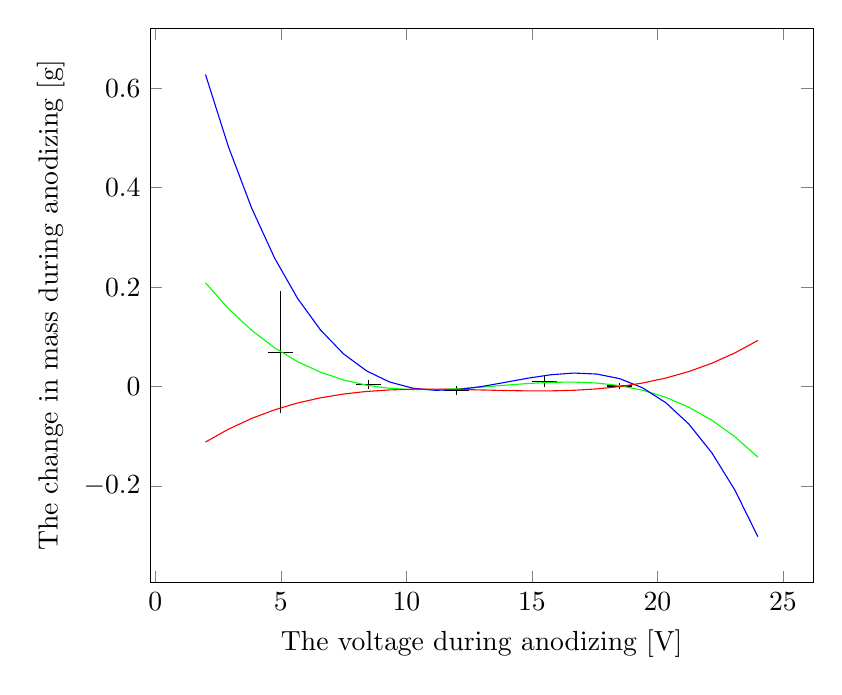
\begin{tikzpicture}
    \begin{axis}[
      xlabel={The voltage during anodizing $[\si{V}]$},
      ylabel={The change in mass during anodizing $[\si{g}]$}
    ]
      \addplot[
        mark=o,
        mark size=0pt,
        only marks
      ]
        plot[
          error bars/.cd,
          x dir=both,
          x explicit,
          y dir=both,
          y explicit
        ] coordinates {
          (5, 0.0695) +- (0.5, 0.1221)
          (8.5, 0.0043) +- (0.5, 0.0088)
          (12, -0.0074) +- (0.5, 0.0084)
          (15.5, 0.0105) +- (0.5, 0.011)
          (18.5, 0.0014) +- (0.5, 0.0061)
        };

        \addplot[domain=2:24, color=green]{-0.0001641 * x^3 + 0.006684 * x^2 -
        0.08666 * x + 0.3567};

        \addplot[domain=2:24, color=blue]{-0.0004155 * x^3 + 0.01755 * x^2 -
        0.2376 * x + 1.036};

        \addplot[domain=2:24, color=red]{0.00008727 * x^3 - 0.003425 * x^2 +
        0.04353 * x - 0.1854};
    \end{axis}
  \end{tikzpicture}
  \caption{The relationship between the voltage and the change in mass}
  \label{fig:voltage-delta}
\end{figure}

\section{Analysis}

\paragraph*{}
The cubic relation indicates that it is impossible to accurately gauge the
thickness of the oxide layer, due to issues presented in section
\ref{sec:accurate-model}.

\paragraph*{}
The relationship also indicates that at one point the process of anodizing
stops adding mass (attributed by the extra addition of oxygen), and rather
starts decreasing the mass of the aluminum. The point at which this effect
comes to be, for a constant time and temperature of anodizing, is given by the
solutions to the given equation:
\begin{align*}
  \Delta m' (V) &= 0 \\
  -4.923 \cdot 10^{-4} V^2 + 13.368 \cdot 10^{-3} V - 8.666 \cdot 10^{-2} &= 0
\end{align*}
These solutions are:
\begin{align*}
  V_1 &= 16.460 \si{V} \\
  V_2 &= 10.965 \si{V}
\end{align*}

\paragraph*{}
At $5\si{min}$ as the time of anodizing, from $V=0\si{V}$ to $V=10.965\si{V}$,
it can be assumed that the film produced is of the barrier type. From
$V=10.965\si{V}$ to $V=16.460\si{V}$, it is likely that the pores start
forming. From $V=16.460\si{V}$ onward, it is most likely that the pores become
deeper, decreasing the resistance, and therefore increasing the rate of
anodizing.

\section{Evaluation}

\paragraph*{}
The obvious issue with the data presented is that the uncertainties are quite
high. The uncertainty of bar $1$ is exceptionally high and to a great extent
skews the data. This outlying uncertainty is most likely due to a systematic
error. The most likely error is due to the measurement conducted after the
anodizing of bar $2$ as it shows an exceptional deviation from the rest. This
systematic error is probably that after the anodizing and the tempering of the
bar it was improperly dried and, therefore, during the weighing process, more
mass was present. As such, it is possible that the data presented is somewhat
invalid.

\paragraph*{}
However, on the other hand, the remaining data has relatively low uncertainties
and can be considered sufficiently precise. It is far more likely that the 

\section{Conclusion}

\paragraph*{}
The data does not prove the original hypothesis as the fit function is a cubic
one:
$$\Delta m (V)_{green} = -1.641 \cdot 10^{-4} V^3 + 6.684 \cdot 10^{-3} V^2 -
  8.666 \cdot 10^{-2} V + 3.567 \cdot 10^{-1}$$
However, this research indicates that the anodizing process does have $4$
separate stages. This reaffirms the research done by Ono.

\paragraph*{}
Overall, this research did not give exact quantitative trends due to the low
precision, however it did show the general qualitative trend of the anodizing
process, with its four distinct stages.

\singlespacing
\clearpage
\pagebreak
\pagenumbering{gobble}
\section*{Works Cited}
\begin{hangparas}{.25in}{1}
  \begin{sloppypar}
    Ardelean, Marius and Lascău, S and Ardelean, Erika and Josan, Ana.
    ``Surface Treatments For Aluminium Alloys''. \textit{IOP Conference Series:
    Materials Science And Engineering}, vol 294, 2018,
    doi:10.1088/1757-899X/294/1/012042.  Accessed 4 Mar 2019. \\

    ``E10K''. \textit{Fiio.Com}, \url{https://www.fiio.com/e10k}. Accessed 4
    Mar 2018. \\

    Fischer. \textit{Anodization}.
    \url{http://www.fischer-technology.com/en/united-states/solutions/galvanization-and-anodization/anodization/}.
    Accessed 4 Mar 2019. \\

    KI. \textit{Clear Anodized Aluminum}. 2019,
    \url{https://www.ki.com/Store/Finishes/Edge/Clear_Anodized_Aluminum.aspx}.
    Accessed 4 Mar 2019. \\

    \textit{Numpy}. 1.16.1, Numpy Developers, 2018. \\

    Ono, Sachiko. ``Structure And Growth Mechanism Of Anodic Oxide Films Formed
    On Aluminum And Their Gas Emission''. Department Of Applied Chemistry,
    Faculty Of Engineering, Kogakuin University,
    \url{http://www.lm-foundation.or.jp/english/abstract-vol43/abstract/12.html}.
    Accessed 4 Mar 2019. \\

    \textit{Python}. Version 3.7.2, Python Software Foundation, 2019. \\

    Sheasby, P. G.; Pinner, R. \textit{The Surface Treatment And Finishing Of
    Aluminum And Its Alloys}. 6th ed., ASM International \& Finishing
    Publications, 2001. \\

    ``Sulfuric Acid''. \textit{Pubchem.Ncbi.Nlm.Nih.Gov},
    \url{https://pubchem.ncbi.nlm.nih.gov/compound/sulfuric_acid#section=Hazards-Identification}.
    Accessed 6 Mar 2019. \\
  \end{sloppypar}
\end{hangparas}

\pagebreak
\section*{Appendices}

\subsection*{Fitting code}

\begin{verbatim}
import numpy as np

V = np.array([5, 8.5, 12, 15.5, 18.5])
V_unc = np.array([0.5, 0.5, 0.5, 0.5, 0.5])

m = np.array([0.0695, 0.0043, -0.0074, 0.0105, 0.0014])
m_unc = np.array([0.1221, 0.0088, 0.0084, 0.011, 0.0061])

V_max = np.add(V, V_unc)
m_max = np.add(m, m_unc)

V_min = np.subtract(V, V_unc)
m_min = np.subtract(m, m_unc)

print(np.poly1d(np.polyfit(V, m, 3)))
print(np.poly1d(np.polyfit(V_max, m_max, 3)))
print(np.poly1d(np.polyfit(V_min, m_min, 3)))
\end{verbatim}

\begin{landscape}

  \begin{table}
    \centering
    \begin{tabular}{l | r | r | r | r | r | r | r | r | r | r | r | r | r | r | r}
       & $1$      & $2$      & $3$      & $4$      & $5$      & $6$      & $7$
       & $8$      & $9$      & $10$     & $11$     & $12$     & $13$     & $14$
       & $15$     \\ \hline \hline $a$ ($\pm 0.01$) [$\si{mm}$]     & $49.80$
       & $47.22$  & $46.80$  & $49.70$  & $49.82$  & $49.80$  & $49.80$  &
       $49.82$  & $49.68$  & $49.62$  & $49.58$  & $49.58$  & $49.0$   &
       $49.62$  & $49.68$  \\ $b$ ($\pm 0.01 $) [$\si{mm}$]    & $20.30$  &
       $20.30$  & $20.30$ & $20.40$  & $20.38$  & $20.10$  & $20.28$  & $20.20$
       & $20.30$  & $20.34$ & $20.28$  & $20.18$  & $20.30$  & $20.20$  &
       $20.22$  \\ $c$ ($\pm 0.01$) [$\si{mm}$]     & $0.72$   & $0.50$   &
       $0.58$   & $0.60$   & $0.62$   & $0.88$   & $0.58$   & $0.55$   & $0.62$
       & $0.48$   & $0.64$   & $0.60$   & $0.50$   & $0.54$   & $0.42$   \\
       $m_{b1}$ ($\pm 0.0001$) [$\si{g}$] & $1.1555$ & $1.1482$ & $1.2061$ &
       $1.1753$ & $1.1432$ & $1.1660$ & $1.1679$ & $1.1599$ & $1.1478$ &
       $1.1292$  & $1.1624$ & $1.1090$ & $1.1065$ & $0.9998$ & $0.9758$ \\
       $m_{b2}$ ($\pm 0.0001$) [$\si{g}$] & $1.1651$ & $1.1462$ & $1.2064$ &
       $1.1752$ & $1.1478$ & $1.1671$ & $1.1697$ & $1.1614$ & $1.1492$ &
       $1.1639$ & $1.1446$ & $1.1107$ & $1.1294$ & $1.0014$ & $0.9759$ \\
       $m_{b3}$ ($\pm 0.0001$) [$\si{g}$] & $1.1720$ & $1.1919$ & $1.1987$ &
       $1.1746$ & $1.1505$ & $1.1673$ & $1.1695$ & $1.1614$ & $1.1559$ &
       $1.1643$ & $1.1034$ & $1.1104$ & $1.0921$ & $0.9996$ & $0.9759$ \\ $V$
       ($\pm 0.1$) [$\si{V}$] & $5.0$    & $5.0$    & $5.0$    & $8.5$    &
       $8.5$    & $8.5$    & $12$ & $12$     & $12$     & $15.5$   & $15.5$   &
       $15.5$   & $18.5$   & $18.5$ & $18.5$   \\ $m_{a1}$ ($\pm 0.0001$)
       [$\si{g}$] & $1.1851$ & $1.1767$ & $1.1875$ & $1.1734$ & $1.1555$ &
       $1.1644$ & $1.1691$ & $1.1582$ & $1.1401$ & $1.1623$ & $1.1431$ &
       $1.1098$ & $1.0910$ & $0.9771$ & $0.9794$ \\ $m_{a2}$ ($\pm 0.0001$)
       [$\si{g}$] & $1.1636$ & $1.1768$ & $1.1888$ & $1.1750$ & $1.1736$ &
       $1.1657$ & $1.1843$ & $1.1588$ & $1.1478$ & $1.1986$ & $1.1450$ &
       $1.1115$ & $1.1106$ & $1.0306$ & $0.9800$ \\ $m_{a3}$ ($\pm 0.0001$)
       [$\si{g}$] & $1.1876$ & $1.7610$ & $1.1887$ & $1.1762$ & $1.1558$ &
       $1.1659$ & $1.1540$ & $1.1161$ & $1.1478$ & $1.1640$ & $1.1467$ &
       $1.1117$ & $1.1098$ & $1.0111$ & $0.9794$ \\
    \end{tabular}
    \caption{The raw data}
    \label{tab:raw-data}
  \end{table}

  \begin{table}[ht]
    \centering
    \begin{tabular}{l | r | r | r| r | r | r | r | r | r | r | r | r | r | r | r}
      $\#$ & $1$ & $2$ & $3$ & $4$ & $5$ & $6$ & $7$ & $8$ & $9$ & $10$ & $11$
      & $12$ & $13$ & $14$ & $15$ \\ \hline \hline
      $V (\pm 0.1) [\si{V}]$ & \multicolumn{3}{r|}{$5$}        &
      \multicolumn{3}{r|}{$8.5$}      & \multicolumn{3}{r|}{$12$}       &
      \multicolumn{3}{r|}{$15.5$}     & \multicolumn{3}{r}{$18.5$}     \\
      \hline
      $\overline{m_b} [\si{g}]$ & $1.1642$ & $1.1621$ & $1.2037$ & $1.1472$ &
      $1.1472$ & $1.1668$ & $1.1690$ & $1.1609$ & $1.1510$ & $1.1525$ &
      $1.1368$ & $1.1100$ & $1.1093$ & $1.0003$ & $0.9759$ \\ $\sigma (m_b)
      [\si{g}]$
      & $0.0083$ & $0.0258$ & $0.0044$ & $0.0004$ & $0.0037$ & $0.0007$ &
      $0.0010$ & $0.0009$ & $0.0043$ & $0.0202$ & $0.0303$ & $0.0009$ &
      $0.0188$ & $0.0010$ & $0.0001$ \\ $\overline{m_a} [\si{g}]$
      & $1.1788$ & $1.3715$ & $1.1883$ & $1.1749$ & $1.1616$ & $1.1653$ &
      $1.1691$ & $1.1444$ & $1.1452$ & $1.1750$ & $1.1449$ & $1.1110$ &
      $1.1038$ & $1.0063$ & $0.9796$ \\ $\sigma (m_a) [\si{g}]$
      & $0.0132$ & $0.3373$ & $0.0007$ & $0.0014$ & $0.0104$ & $0.0008$ &
      $0.0152$ & $0.0245$ & $0.0044$ & $0.0205$ & $0.0018$ & $0.0010$ &
      $0.0111$ & $0.0271$ & $0.0003$ \\ $\Delta \overline{m} [\cdot 10^{-3}
      \si{g}]$
      & $14.6$ & $209.4$  & $-15.4$  & $-0.1$   & $14.4$   & $-1.5$   & $0.1$
      & $-16.5$  & $-5.8$   & $22.5$   & $8.1$    & $1.0$    & $-5.5$   & $6.0$
      & $3.7$    \\ $\mu (\Delta \overline{m}) [\cdot 10^{-3} \si{g}]$    &
      $21.5$   &
      $36.31$  & $5.1$    & $1.8$    & $14.1$   & $1.5$    & $16.2$   & $25.4$
      & $8.7$    & $40.7$   & $32.1$   & $1.9$    & $29.9$   & $28.1$   & $0.4$
      \\ \hline $\overline{\Delta \overline{m}} [\cdot 10^{-3} \si{g}]$    &
      \multicolumn{3}{r|}{$69.5$} & \multicolumn{3}{r|}{$4.3$}      &
      \multicolumn{3}{r|}{$-7.4$}     & \multicolumn{3}{r|}{$10.5$}     &
      \multicolumn{3}{r}{$1.4$}      \\ \hline $\sigma (\Delta \overline{m}) [\cdot
      10^{-3} \si{g}]$ & \multicolumn{3}{r|}{$122.1$} & \multicolumn{3}{r|}{$8.8$}
      & \multicolumn{3}{r|}{$8.4$}      & \multicolumn{3}{r|}{$11.0$}     &
      \multicolumn{3}{r}{$6.1$}     
    \end{tabular}
    \caption{The processed data}
    \label{tab:processed}
  \end{table}
\end{landscape}

\end{document}
